\documentclass[a4paper,10pt]{article}
\usepackage[top=0.5in, bottom=1in, left=1in, right=1in]{geometry}
\usepackage[utf8]{inputenc}
\usepackage{mathptmx}  % Times New Roman font style
\usepackage{setspace}
\usepackage{titlesec}
\usepackage{hyperref}
\usepackage{graphicx} % For including images

\onehalfspacing  % Set line spacing to 1.5

% Customize section titles
\titleformat{\section}{\normalsize\bfseries}{\thesection.}{1em}{}
\titleformat{\subsection}{\normalsize\bfseries}{\thesubsection.}{1em}{}
\titleformat{\subsubsection}{\normalsize\itshape}{\thesubsubsection.}{1em}{}

% Redefine \maketitle to adjust title and author formatting
\makeatletter
\renewcommand{\maketitle}{
  \begin{center}
    {\fontsize{12pt}{14pt}\selectfont\bfseries\@title\par}
    \vskip 1em
    {\normalsize\@author\par}
    \vskip 1em
  \end{center}
}
\makeatother

\title{Self-Adaptive Systems: Methodologies for Reusability and Security}
\author{Mutasem Salloum (ms227fm) \\ Rashed Qazizada (rq222ah)}
\date{}

\begin{document}

\maketitle

\begin{abstract}
This report investigates two core research questions: (1) What are the current methodologies and approaches for achieving reusability in self-adaptive software systems (SAS)? and (2) What are the benefits and challenges of implementing reusable components in these systems? We examine frameworks such as Autonomic Software Product Line Engineering (ASPLe) and code-level adaptation methods to understand how SAS can be made adaptable and secure. ASPLe supports modularity and flexibility, while code-level strategies enhance adaptability at a granular level. Our findings indicate that reusability reduces development costs and increases resilience. However, the lack of integrated security measures presents risks, especially in critical environments. This study highlights the need for adaptable, security-conscious frameworks that evolve with system requirements, providing a foundation for future research to enhance the security and effectiveness of reusable SAS components.
\end{abstract}

\section{Introduction}

As modern software systems grow in complexity, there is a rising demand for systems that can adapt autonomously to dynamic conditions. Self-adaptive systems (SAS) are designed to meet this need, allowing software to monitor, analyse, and adjust its behaviour based on environmental changes without human intervention. In critical areas such as healthcare, cloud computing, and autonomous vehicles, this capability is essential to maintain continuous functionality despite shifting requirements or unexpected conditions. Achieving this adaptability efficiently requires the reuse of modular components that can be applied across various contexts, reducing both development time and costs.

This report investigates two research questions central to the advancement of SAS:

\begin{itemize}
    \item \textbf{RQ1:} What are the current methodologies and approaches used to achieve reusability in self-adaptive software systems?
    \item \textbf{RQ2:} What are the benefits and challenges of implementing reusable components in self-adaptive software systems?
\end{itemize}

To address these questions, we need to understand a few concepts:

\begin{itemize}
    \item \textbf{Self-Adaptive Software System (SASS):} A system that can modify its behaviour and structure in response to changes in its environment, its own internal state, or its goals.
    
    \item \textbf{ASPLe (Autonomic Software Product Line Engineering):} ASPLe organizes SAS development into domain engineering, specialization, and integration stages, promoting systematic reuse of components across different applications. This modular approach saves time and supports consistent quality by allowing components to be adapted with minimal effort.
    
    \item \textbf{Code-level adaptation methods:} This strategy focuses on reusability at the coding level, allowing adaptation within specific modules. Code-level adaptation enables flexibility on a smaller scale, complementing the higher-level reusability of frameworks like ASPLe, though it may encounter scalability challenges in larger systems.
    
%     \item \textbf{MAPE-K (Monitor-Analyze-Plan-Execute with Knowledge):} MAPE-K emphasizes real-time adaptability, enabling SAS to continuously assess and adjust their actions based on feedback from their environment. This feedback loop approach offers flexibility but lacks integrated security, raising concerns for systems operating in sensitive environments.
\end{itemize}

The motivation behind these research questions stems from the need to balance adaptability and security in SAS. While reusability can enhance efficiency and resilience, it can also expose systems to potential vulnerabilities if security measures are not integrated within the reusable components. This report provides insights into these challenges and suggests future directions for enhancing SAS with more secure and flexible reusable components, offering a foundation for further research on building robust adaptive systems that can evolve with changing conditions.

\section{Approach or Method}

To explore and answer the research questions, we conducted a systematic literature review (SLR), focusing on recent studies related to self-adaptive systems (SAS), particularly those emphasizing modularity, reuse, and adaptive security. In alignment with the project’s requirements, all articles were selected from Norwegian List Level 2 journals, ensuring a high standard of peer-reviewed quality and relevance in the field.

\subsection{Systematic Literature Review}

The SLR involved a structured search across academic databases, including IEEE Xplore, ScienceDirect, and SpringerLink. The search terms used were “self-adaptive systems,” “systematic reuse,” and “security.” Articles were chosen based on their alignment with the research questions, publication date (2020–2024), and relevance to SAS reusability. This selection process resulted in three primary sources:

\begin{enumerate}
    \item \textbf{ASPLe:} A methodology for reuse in self-adaptive systems, detailing a structured approach for developing reusable components \cite{Nadeem2020}.
    
    \item \textbf{Systematic review on security and safety in SAS:} This article highlights the security challenges in adaptive systems, especially in high-risk environments \cite{Pekaric2023}.
    
    \item \textbf{Code-level adaptation for SAS:} This source explores code-level techniques to enhance flexibility and adaptability within SAS, complementing broader reuse strategies \cite{Korra2022}.
\end{enumerate}

\subsection{Analyzing Methodologies}

Each methodology was analyzed for its approach to modularity, adaptability, and security:

\begin{itemize}
    \item \textbf{ASPLe (Autonomic Software Product Line Engineering):} Detailed in the work on ASPLe, this methodology divides SAS development into domain engineering, specialization, and integration stages, creating modular artifacts for reuse. This approach supports consistent quality and adaptability across different SAS applications \cite{Nadeem2020}.
    
    % \item \textbf{MAPE-K (Monitor-Analyze-Plan-Execute with Knowledge):} Discussed in the context of adaptive systems security, the MAPE-K model uses a feedback loop to continuously adapt SAS based on environmental feedback. While MAPE-K supports dynamic adaptability, it lacks integrated security measures, posing potential risks in sensitive applications \cite{Pekaric2023}.
    
    \item \textbf{Code-Level Adaptation Techniques:} Described in research on code-level approaches, this method focuses on adaptable coding practices to enable flexibility at a more granular level. Code-level adaptation is particularly beneficial for implementing fine-grained adjustments within specific modules, complementing the broader reuse strategy provided by frameworks like ASPLe \cite{Korra2022}.
\end{itemize}

This approach is suitable as it provides a comprehensive view of modularity, adaptability, and security concerns essential to effectively answering RQ1 and RQ2.


% \section{Results}

% This section presents the findings related to the research questions on reusable methodologies in self-adaptive systems (SAS). The results focus on the ASPL strategy and ASPLe methodology, the proposed algorithm for adaptive component development, and the component metrics used for evaluation.

% \subsection{ASPL Strategy and ASPLe Methodology}

% The \textbf{Autonomic Software Product Lines (ASPL)} strategy addresses key challenges in software development related to variability, reuse, and uncertainty. It is based on two fundamental principles: (1) strict separation of managed and managing system concerns, and (2) stepwise specialization of reusable assets into product-specific assets. These principles reduce complexity and mitigate uncertainty in the development process \cite{Nadeem2020}.

% The ASPL strategy consists of three steps:

% \begin{enumerate}
%     \item \textbf{Establish a Horizontal ASPL Platform}: Create a horizontal platform with domain-independent artifacts reusable across multiple managing subsystems. These artifacts cover all stages of the development lifecycle and are designed for reuse across various domains.

%     \item \textbf{Derive a Vertical Managing System Platform}: Transform the horizontal platform into vertical managing system platforms tailored to the adaptation logic of specific application domains.

%     \item \textbf{Integrate Platforms}: Integrate the managing system platform with a separately developed managed system platform containing the application logic, developed using approaches like Software Product Line Engineering (SPLE).
% \end{enumerate}

% While the ASPL strategy is critical for developing SAS, it faces a significant research gap due to the lack of detailed process support for engineers to apply the strategy consistently in real-world projects.

% To address this gap, the \textbf{ASPLe (Autonomic Software Product Line Engineering)} methodology was developed. It provides process support for systematic reuse at the managing system level, aligned with the ASPL strategy. ASPLe is organized into three primary processes: \textit{ASPL Domain Engineering}, \textit{Specialization}, and \textit{Integration}. A key element of ASPLe is the \textbf{Extended Architectural Reasoning Framework (eARF)}, which incorporates design support for self-adaptive properties like self-healing and self-optimization. The eARF guides domain analysts and designers through a structured process of identifying and specifying self-adaptation requirements using domain Quality Attribute Scenarios (dQAS) and mapping these requirements to design alternatives. It leverages reusable architectural tactics and patterns to ensure that design decisions are well-founded and aligned with quality attributes. This facilitates the development of flexible, adaptable systems capable of accommodating changes in dynamic environments \cite{Nadeem2020}.

% % Insert a diagram here
% \begin{figure}[h]
% \centering
% 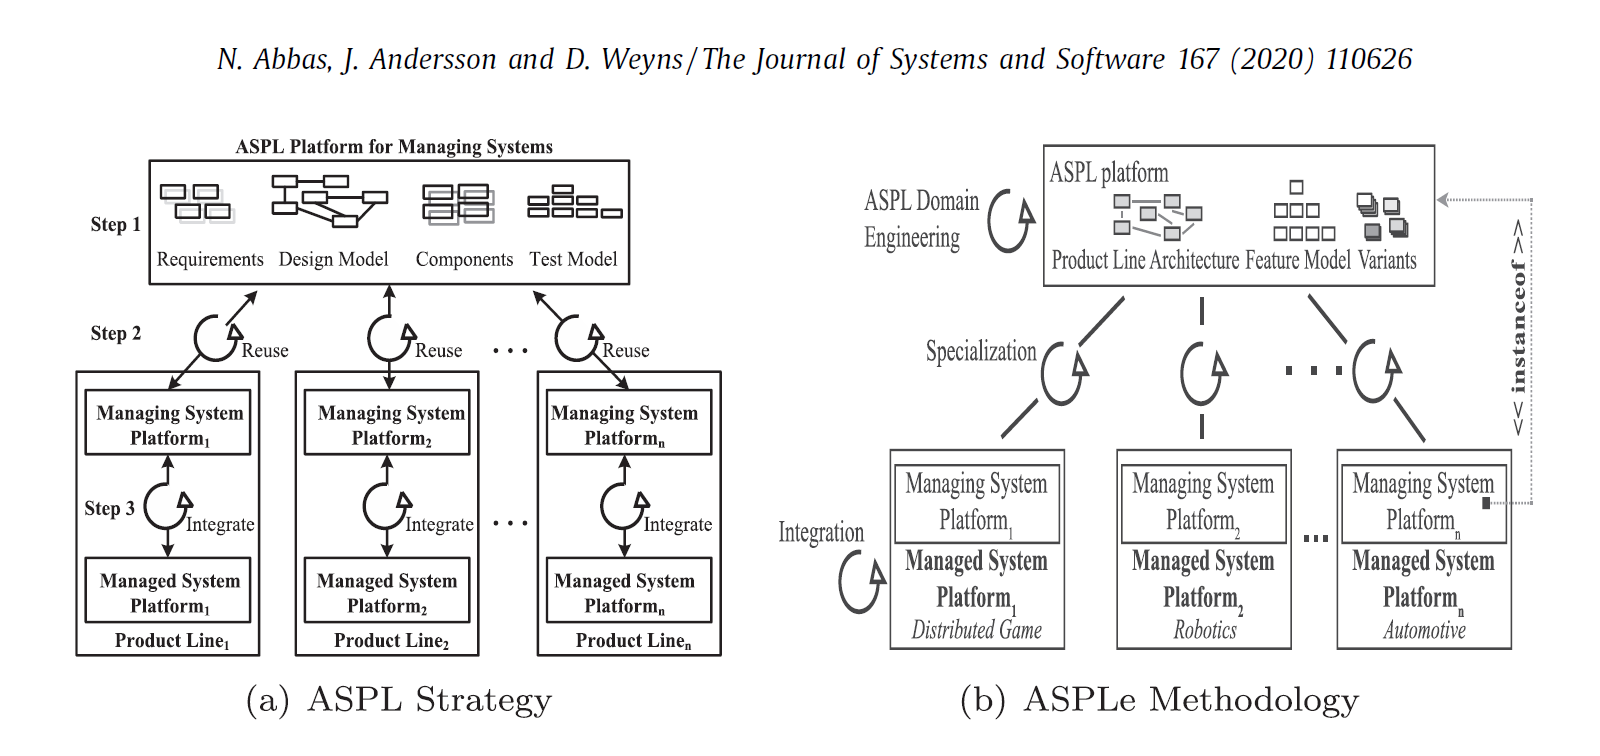
\includegraphics[width=0.8\textwidth]{asple_diagram.png}
% \caption{ASPLe Methodology Overview}
% \label{fig:asple}
% \end{figure}


% \textbf{Benefits and Challenges}:

% The ASPL strategy and ASPLe methodology offer several benefits. They **reduce complexity** by separating managed and managing system concerns, making systems easier to manage and evolve over time. **Systematic reuse** is promoted by reusing artifacts across multiple domains, which reduces development time and costs. **Scalability** is enhanced by deriving domain-specific platforms from a horizontal platform, enabling efficient expansion. **Flexibility in design** is achieved through stepwise specialization of reusable assets into product-specific assets, facilitating customization without starting from scratch.

% However, challenges exist in their implementation. A significant **research gap in methodology** hinders consistent application in real-world projects due to the lack of detailed process support for engineers. **Complex integration** of managed and managing system platforms can be challenging, especially with diverse software components and technologies. Additionally, **domain-specific customization** may require significant effort, potentially affecting consistency and increasing redundancy across domains.


% \subsection{Proposed Algorithm for Adaptive Component Development}

% The algorithm proposed by Korra et al. \cite{Korra2022} outlines a systematic approach for developing adaptive software components intended for reuse. The primary goal is to enhance efficiency and reduce development time by reusing components across different projects. The algorithm consists of the following steps:

% \begin{enumerate}
%     \item \textbf{Component Identification}: Analyze the software system to identify potential components for reuse by isolating modules that perform distinct operations.

%     \item \textbf{Metric Evaluation}: Apply specific component metrics to evaluate the identified components' suitability for reuse. Metrics such as CEM, CSEM, CRM, CFM, and CCSM assess attributes like efficiency, reliability, functionality, customer satisfaction, and cost.

%     \item \textbf{Component Adaptation}: Modify components as necessary to meet adaptability criteria, which may involve refactoring code or enhancing interfaces to ensure compatibility across different systems.

%     \item \textbf{Component Documentation}: Provide comprehensive documentation for each component, including usage guidelines, interfaces, and dependencies, to facilitate integration and reuse.

%     \item \textbf{Repository Management}: Store reusable components in a centralized repository with appropriate categorization and metadata for efficient retrieval and management.

%     \item \textbf{Integration and Testing}: Integrate components into new projects and conduct rigorous testing to verify their functionality and adaptability in different contexts.
% \end{enumerate}

% \subsection{Component Metrics for Evaluation}

% To effectively evaluate and select components for reuse, the following metrics are introduced:

% \begin{itemize}
%     \item \textbf{Component Efficiency Metrics (CEM)}: Measure performance in terms of execution time and resource utilization.

%     \item \textbf{Component Semantic Efficiency Measurement (CSEM)}: Assess efficiency from a semantic perspective, including code readability, maintainability, and adherence to coding standards.

%     \item \textbf{Component Reliability Metrics (CRM)}: Estimate the probability of functioning without defects over a specified period, critical for safety-critical systems.

%     \item \textbf{Component Functional Metrics (CFM)}: Evaluate functionality, precision, interoperability, and suitability for the intended purpose.

%     \item \textbf{Component Customer Satisfaction Measurement (CCSM)}: Gauge the extent to which components meet user expectations, based on feedback and satisfaction surveys.

%     \item \textbf{Component Cost Metrics (CCM)}: Account for costs associated with development, acquisition, and integration, aiding in assessing economic viability.
% \end{itemize}
% \textbf{Benefits and Challenges}:

% The ASPL strategy and ASPLe methodology offer several benefits. They \textbf{reduce complexity} by separating managed and managing system concerns, making systems easier to manage and evolve over time. \textbf{Systematic reuse} is promoted by reusing artifacts across multiple domains, which reduces development time and costs. \textbf{Scalability} is enhanced by deriving domain-specific platforms from a horizontal platform, enabling efficient expansion. \textbf{Flexibility in design} is achieved through stepwise specialization of reusable assets into product-specific assets, facilitating customization without starting from scratch.

% However, challenges exist in their implementation. A significant \textbf{research gap in methodology} hinders consistent application in real-world projects due to the lack of detailed process support for engineers. \textbf{Complex integration} of managed and managing system platforms can be challenging, especially with diverse software components and technologies. Additionally, \textbf{domain-specific customization} may require significant effort, potentially affecting consistency and increasing redundancy across domains.


% \subsection{Benefits and Challenges of the Proposed Algorithm}
    
% The proposed algorithm offers several benefits. It focuses on \textbf{component reusability}, promoting code reuse and reducing the need for new development, thereby speeding up project timelines. \textbf{Efficiency and cost savings} are achieved by leveraging pre-existing, well-tested components, which reduces overall development time and costs. The algorithm ensures \textbf{component compatibility} by using metrics like CEM, CSEM, and CRM to select components that meet specific adaptability criteria, enhancing system performance and reliability. Additionally, the use of a \textbf{centralized repository} simplifies component management and retrieval, facilitating easy access and integration into new projects.

% However, there are challenges in implementing the algorithm. \textbf{Initial component identification} requires significant analysis and abstraction, particularly in large or legacy systems. \textbf{Adaptation complexity} arises when modifying components to fit different systems or contexts, often necessitating substantial refactoring or interface changes. The \textbf{evaluation of multiple metrics} may not always provide clear guidance, especially when components interact unexpectedly or when system requirements evolve rapidly. Ensuring components function correctly across different contexts requires rigorous testing, leading to \textbf{testing and integration overhead}. Finally, \textbf{dependency management} becomes increasingly complex as the number of components grows, making compatibility and version control challenging.


% \section{Discussion}

% The findings underscore the practical benefits and challenges associated with implementing reusable components in self-adaptive systems (SAS). This discussion interprets the results, reflects on their implications, and suggests areas for future research.

% \subsection{Interpretation of Results}

% The successful application of the ASPL strategy and the ASPLe methodology demonstrates the effectiveness of systematic reuse in SAS development. By separating managed and managing system concerns and employing stepwise specialization, organizations can reduce complexity and promote scalability and flexibility in design. The use of the eARF within ASPLe aids in aligning design decisions with quality attributes, facilitating the development of adaptable systems.

% The proposed algorithm for adaptive component development complements these methodologies by providing a practical approach to identifying, evaluating, and adapting components for reuse. The incorporation of comprehensive metrics ensures that components meet specific criteria for efficiency, reliability, and functionality, which is crucial for maintaining high performance and user satisfaction.

% \subsection{Implications for Practice}

% Implementing these methodologies and algorithms can lead to more efficient software development processes, particularly in domains where adaptability and reliability are critical. Organizations can benefit from reduced development time and costs by reusing well-tested components. The establishment of centralized repositories and the use of metrics promote a culture of quality and continuous improvement.

% However, the challenges identified, such as the initial effort required for component identification and adaptation complexity, suggest that organizations need to invest in developing expertise and tools to support these processes. The lack of detailed process support in the ASPL strategy indicates a need for further refinement of methodologies like ASPLe to facilitate their practical application.

% \subsection{Comparison with Existing Literature}

% These findings align with existing research emphasizing the importance of modularity and reuse in software engineering. The ASPLe methodology extends traditional software product line engineering by incorporating self-adaptive properties, addressing a gap noted in prior studies \cite{Nadeem2020}. The proposed algorithm adds value by focusing on code-level adaptation, complementing higher-level strategies.

% \subsection{Limitations and Future Work}

% Despite the benefits, several limitations exist. The current metrics do not explicitly address security concerns, which is critical in sensitive applications. Additionally, evaluating components using multiple metrics can be time-consuming, and the integration of components may present unforeseen challenges due to dependencies.

% Future work should focus on integrating security metrics into the evaluation framework to address potential vulnerabilities. Developing automated tools to streamline the evaluation process could reduce the time and effort required. Customizing metrics for different domains would enhance their relevance and effectiveness, and enhancing documentation could mitigate integration issues.

% % End of Discussion section

% \section{Conclusion}

% This study explored methodologies for reusability in self-adaptive systems (SAS), focusing on the ASPL strategy, the ASPLe methodology, and a proposed algorithm for adaptive component development. By introducing systematic approaches and comprehensive metrics for component evaluation, the study demonstrated that careful selection and development of components enhance adaptability, cost efficiency, and reliability in SAS.

% Key findings include that reusing components evaluated through specific metrics leads to significant reductions in development time and costs, and that components selected based on efficiency, reliability, and functionality maintain high performance and user satisfaction in new systems. However, challenges such as the lack of integrated security measures and scalability issues highlight the need for further research.

% By addressing these challenges, the methodologies and algorithms can be refined to build more adaptable, secure, and efficient self-adaptive systems that meet the evolving demands of various industries.

% \section{Results}

% This section presents the findings related to the research questions on reusable methodologies in self-adaptive systems (SAS). The results focus on the ASPL strategy and ASPLe methodology, the MAPE-K model, the proposed algorithm for adaptive component development, and the component metrics used for evaluation.

% \subsection{ASPL Strategy and ASPLe Methodology}

% The \textbf{Autonomic Software Product Lines (ASPL)} strategy addresses key challenges in software development related to variability, reuse, and uncertainty. It is based on two fundamental principles: (1) strict separation of managed and managing system concerns, and (2) stepwise specialization of reusable assets into product-specific assets. These principles reduce complexity and mitigate uncertainty in the development process \cite{Nadeem2020}.

% The ASPL strategy consists of three steps:

% \begin{enumerate}
%     \item \textbf{Establish a Horizontal ASPL Platform}: Create a horizontal platform with domain-independent artifacts reusable across multiple managing subsystems. These artifacts cover all stages of the development lifecycle and are designed for reuse across various domains.

%     \item \textbf{Derive a Vertical Managing System Platform}: Transform the horizontal platform into vertical managing system platforms tailored to the adaptation logic of specific application domains.

%     \item \textbf{Integrate Platforms}: Integrate the managing system platform with a separately developed managed system platform containing the application logic, developed using approaches like Software Product Line Engineering (SPLE).
% \end{enumerate}

% While the ASPL strategy is critical for developing SAS, it faces a significant research gap due to the lack of detailed process support for engineers to apply the strategy consistently in real-world projects.

% To address this gap, the \textbf{ASPLe (Autonomic Software Product Line Engineering)} methodology was developed. It provides process support for systematic reuse at the managing system level, aligned with the ASPL strategy. ASPLe is organized into three primary processes: \textit{ASPL Domain Engineering}, \textit{Specialization}, and \textit{Integration}. A key element of ASPLe is the \textbf{Extended Architectural Reasoning Framework (eARF)}, which incorporates design support for self-adaptive properties like self-healing and self-optimization. The eARF guides domain analysts and designers through a structured process of identifying and specifying self-adaptation requirements using domain Quality Attribute Scenarios (dQAS) and mapping these requirements to design alternatives. It leverages reusable architectural tactics and patterns to ensure that design decisions are well-founded and aligned with quality attributes. This facilitates the development of flexible, adaptable systems capable of accommodating changes in dynamic environments \cite{Nadeem2020}.

% % Insert a diagram here
% \begin{figure}[h]
% \centering
% 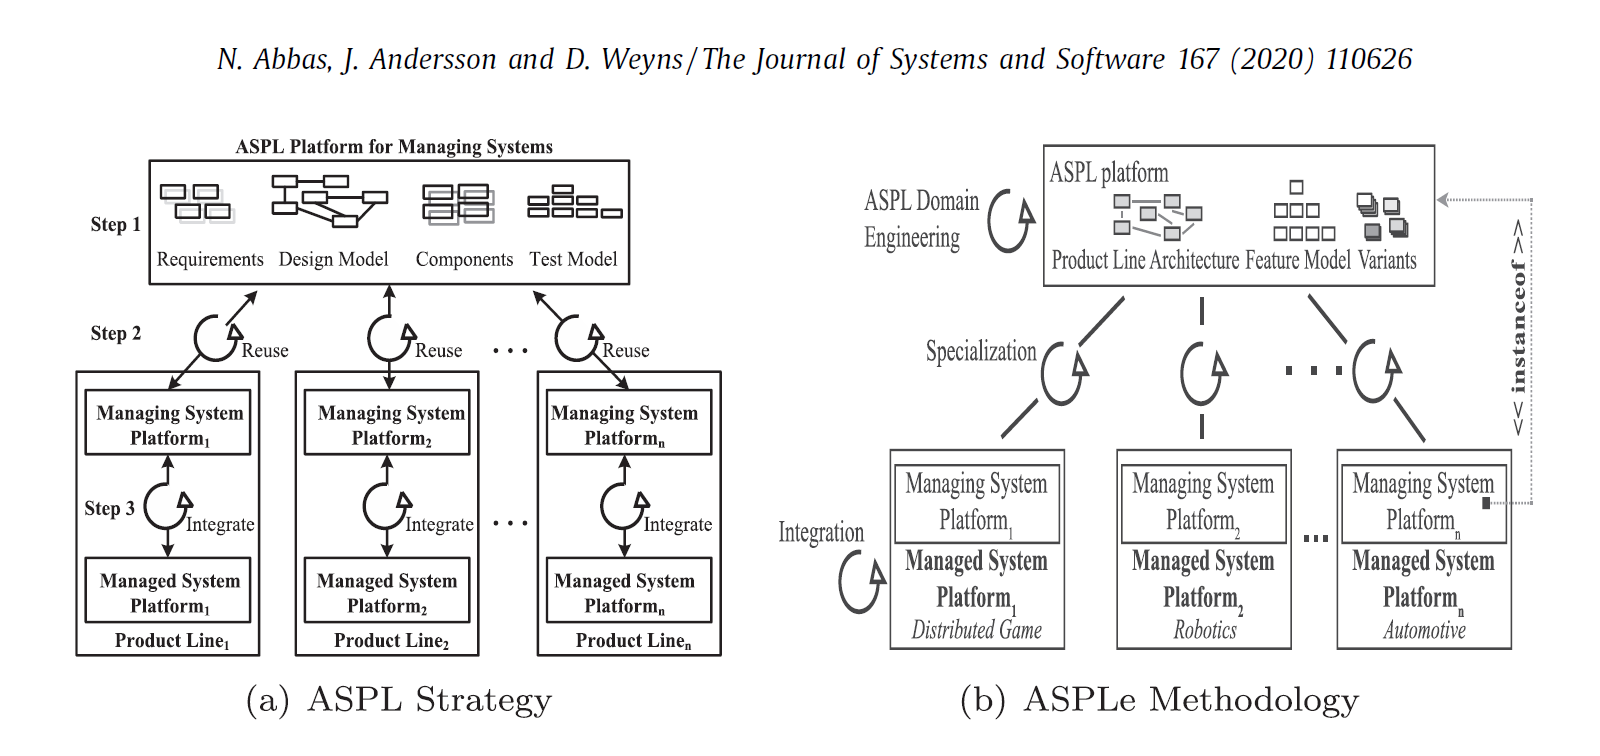
\includegraphics[width=0.8\textwidth]{asple_diagram.png}
% \caption{ASPLe Methodology Overview}
% \label{fig:asple}
% \end{figure}

% \textbf{Benefits and Challenges}:

% The ASPL strategy and ASPLe methodology offer several benefits. They \textbf{reduce complexity} by separating managed and managing system concerns, making systems easier to manage and evolve over time. \textbf{Systematic reuse} is promoted by reusing artifacts across multiple domains, which reduces development time and costs. \textbf{Scalability} is enhanced by deriving domain-specific platforms from a horizontal platform, enabling efficient expansion. \textbf{Flexibility in design} is achieved through stepwise specialization of reusable assets into product-specific assets, facilitating customization without starting from scratch.

% However, challenges exist in their implementation. A significant \textbf{research gap in methodology} hinders consistent application in real-world projects due to the lack of detailed process support for engineers. \textbf{Complex integration} of managed and managing system platforms can be challenging, especially with diverse software components and technologies. Additionally, \textbf{domain-specific customization} may require significant effort, potentially affecting consistency and increasing redundancy across domains.

% \subsection{MAPE-K Model}

% The \textbf{Monitor-Analyze-Plan-Execute over a shared Knowledge (MAPE-K)} model is a commonly used framework for developing self-adaptive systems \cite{Cheng2009}. It provides a structured feedback loop where the system continuously monitors its environment, analyzes changes, plans appropriate responses, and executes those plans, all while maintaining a shared knowledge base.

% \textbf{Benefits and Challenges}:

% MAPE-K offers significant benefits in terms of dynamic adaptability and real-time responsiveness. Its modular structure allows for scalability and flexibility in design. However, it lacks integrated security measures, posing potential risks, especially in sensitive applications \cite{Pekaric2023}. Addressing security within MAPE-K requires additional layers, which can increase system complexity and development efforts.

% \subsection{Proposed Algorithm for Adaptive Component Development}

% The algorithm proposed by Korra et al. \cite{Korra2022} outlines a systematic approach for developing adaptive software components intended for reuse. The primary goal is to enhance efficiency and reduce development time by reusing components across different projects. The algorithm consists of the following steps:

% \begin{enumerate}
%     \item \textbf{Component Identification}: Analyze the software system to identify potential components for reuse by isolating modules that perform distinct operations.

%     \item \textbf{Metric Evaluation}: Apply specific component metrics to evaluate the identified components' suitability for reuse. Metrics such as CEM, CSEM, CRM, CFM, and CCSM assess attributes like efficiency, reliability, functionality, customer satisfaction, and cost.

%     \item \textbf{Component Adaptation}: Modify components as necessary to meet adaptability criteria, which may involve refactoring code or enhancing interfaces to ensure compatibility across different systems.

%     \item \textbf{Component Documentation}: Provide comprehensive documentation for each component, including usage guidelines, interfaces, and dependencies, to facilitate integration and reuse.

%     \item \textbf{Repository Management}: Store reusable components in a centralized repository with appropriate categorization and metadata for efficient retrieval and management.

%     \item \textbf{Integration and Testing}: Integrate components into new projects and conduct rigorous testing to verify their functionality and adaptability in different contexts.
% \end{enumerate}

% \textbf{Benefits and Challenges}:

% The proposed algorithm offers several benefits. It focuses on \textbf{component reusability} promoting code reuse and reducing the need for new development, thereby speeding up project timelines. \textbf{Efficiency and cost savings} are achieved by leveraging pre-existing, well-tested components, which reduces overall development time and costs. The algorithm ensures \textbf{component compatibility} by using metrics like CEM, CSEM, and CRM to select components that meet specific adaptability criteria, enhancing system performance and reliability. Additionally, the use of a \textbf{centralized repository} simplifies component management and retrieval, facilitating easy access and integration into new projects.

% However, there are challenges in implementing the algorithm. \textbf{Initial component identification} requires significant analysis and abstraction, particularly in large or legacy systems. \textbf{Adaptation complexity} arises when modifying components to fit different systems or contexts, often necessitating substantial refactoring or interface changes. The \textbf{evaluation of multiple metrics} may not always provide clear guidance, especially when components interact unexpectedly or when system requirements evolve rapidly. Ensuring components function correctly across different contexts requires rigorous testing, leading to \textbf{testing and integration overhead} Finally, \textbf{dependency management} becomes increasingly complex as the number of components grows, making compatibility and version control challenging.

% \subsection{Component Metrics for Evaluation}

% To effectively evaluate and select components for reuse, the following metrics are introduced:

% \begin{itemize}
%     \item \textbf{Component Efficiency Metrics (CEM)}: Measure performance in terms of execution time and resource utilization.

%     \item \textbf{Component Semantic Efficiency Measurement (CSEM)}: Assess efficiency from a semantic perspective, including code readability, maintainability, and adherence to coding standards.

%     \item \textbf{Component Reliability Metrics (CRM)}: Estimate the probability of functioning without defects over a specified period, critical for safety-critical systems.

%     \item \textbf{Component Functional Metrics (CFM)}: Evaluate functionality, precision, interoperability, and suitability for the intended purpose.

%     \item \textbf{Component Customer Satisfaction Measurement (CCSM)}: Gauge the extent to which components meet user expectations, based on feedback and satisfaction surveys.

%     \item \textbf{Component Cost Metrics (CCM)}: Account for costs associated with development, acquisition, and integration, aiding in assessing economic viability.
% \end{itemize}


\section{Results}

This section presents the findings related to the research questions on reusable methodologies in self-adaptive systems (SAS). The results focus on the ASPL strategy and ASPLe methodology, the proposed algorithm for adaptive component development, and the component metrics used for evaluation. 

\subsection{ASPL Strategy and ASPLe Methodology}

The \textbf{Autonomic Software Product Lines (ASPL)} strategy addresses key challenges in software development related to variability, reuse, and uncertainty. It is based on two fundamental principles: (1) strict separation of managed and managing system concerns, and (2) stepwise specialization of reusable assets into product-specific assets. These principles reduce complexity and mitigate uncertainty in the development process \cite{Nadeem2020}.

The ASPL strategy consists of three steps:

\begin{enumerate}
    \item \textbf{Establish a Horizontal ASPL Platform}: Create a horizontal platform with domain-independent artifacts reusable across multiple managing subsystems. These artifacts cover all stages of the development lifecycle and are designed for reuse across various domains.

    \item \textbf{Derive a Vertical Managing System Platform}: Transform the horizontal platform into vertical managing system platforms tailored to the adaptation logic of specific application domains.

    \item \textbf{Integrate Platforms}: Integrate the managing system platform with a separately developed managed system platform containing the application logic, developed using approaches like Software Product Line Engineering (SPLE).
\end{enumerate}

While the ASPL strategy is critical for developing SAS, it faces a significant research gap due to the lack of detailed process support for engineers to apply the strategy consistently in real-world projects.

To address this gap, the \textbf{ASPLe (Autonomic Software Product Line Engineering)} methodology was developed. It provides process support for systematic reuse at the managing system level, aligned with the ASPL strategy. ASPLe is organized into three primary processes: \textit{ASPL Domain Engineering}, \textit{Specialization}, and \textit{Integration}. A key element of ASPLe is the \textbf{Extended Architectural Reasoning Framework (eARF)}, which incorporates design support for self-adaptive properties like self-healing and self-optimization. The eARF guides domain analysts and designers through a structured process of identifying and specifying self-adaptation requirements using domain Quality Attribute Scenarios (dQAS) and mapping these requirements to design alternatives. It leverages reusable architectural tactics and patterns to ensure that design decisions are well-founded and aligned with quality attributes. This facilitates the development of flexible, adaptable systems capable of accommodating changes in dynamic environments \cite{Nadeem2020}.

% Insert a diagram here
\begin{figure}[h]
\centering
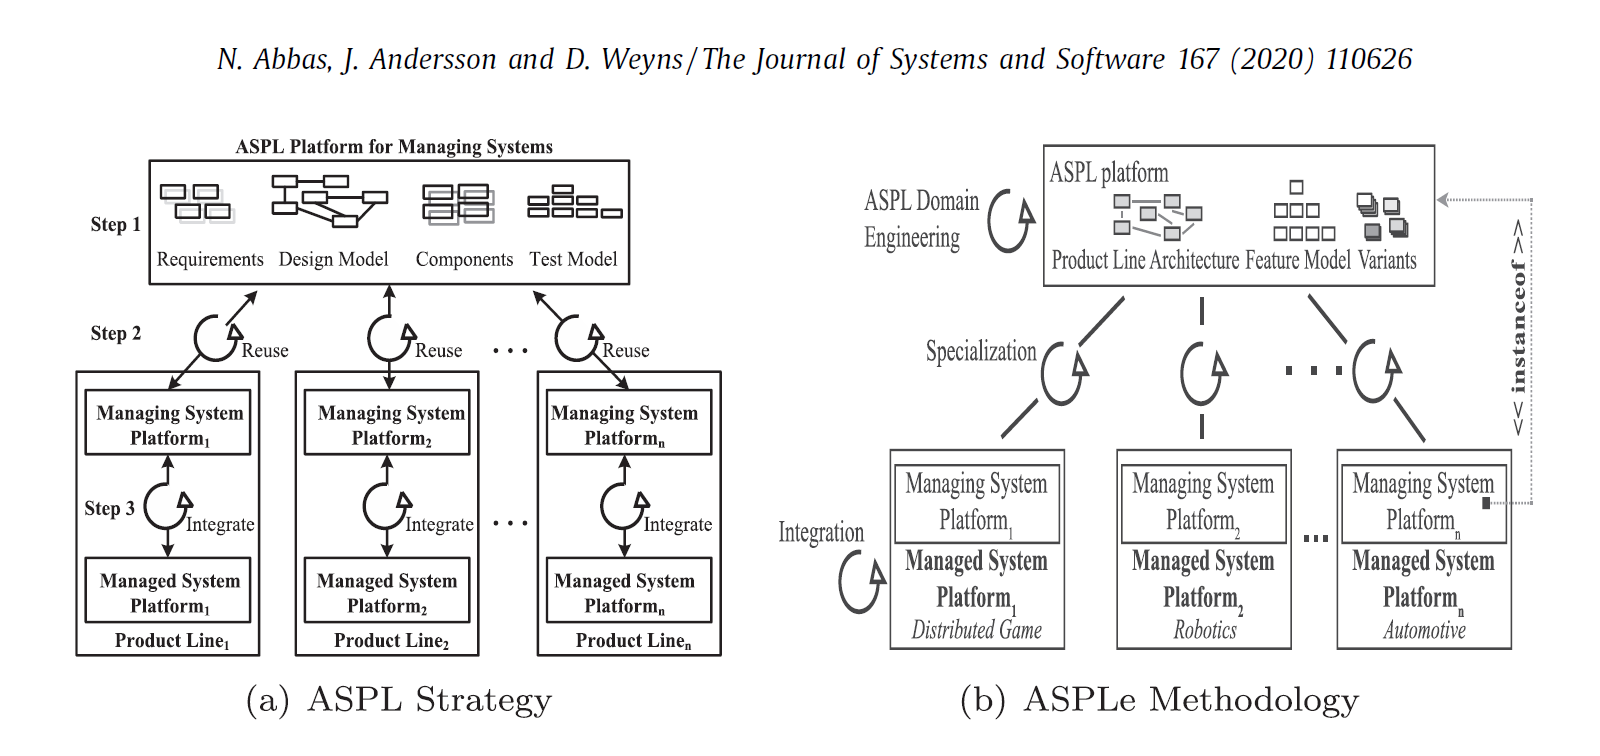
\includegraphics[width=0.8\textwidth]{asple_diagram.png}
\caption{ASPLe Methodology Overview}
\label{fig:asple}
\end{figure}

\textbf{Benefits and Challenges}:

The ASPL strategy and ASPLe methodology offer several benefits. They \textbf{reduce complexity} by separating managed and managing system concerns, making systems easier to manage and evolve over time. \textbf{Systematic reuse} is promoted by reusing artifacts across multiple domains, which reduces development time and costs. \textbf{Scalability} is enhanced by deriving domain-specific platforms from a horizontal platform, enabling efficient expansion. \textbf{Flexibility in design} is achieved through stepwise specialization of reusable assets into product-specific assets, facilitating customization without starting from scratch.

However, challenges exist in their implementation. A significant \textbf{research gap in methodology} hinders consistent application in real-world projects due to the lack of detailed process support for engineers. \textbf{Complex integration} of managed and managing system platforms can be challenging, especially with diverse software components and technologies. Additionally, \textbf{domain-specific customization} may require significant effort, potentially affecting consistency and increasing redundancy across domains.

% \subsection{MAPE-K Model}

% The \textbf{Monitor-Analyze-Plan-Execute over a shared Knowledge (MAPE-K)} model is a commonly used framework for developing self-adaptive systems \cite{Cheng2009}. It provides a structured feedback loop where the system continuously monitors its environment, analyzes changes, plans appropriate responses, and executes those plans, all while maintaining a shared knowledge base.

% \textbf{Benefits and Challenges}:

% MAPE-K offers significant benefits in terms of dynamic adaptability and real-time responsiveness. Its modular structure allows for scalability and flexibility in design. However, it lacks integrated security measures, posing potential risks, especially in sensitive applications \cite{Pekaric2023}. Addressing security within MAPE-K requires additional layers, which can increase system complexity and development efforts.

\subsection{Proposed Algorithm for Adaptive Component Development}

The algorithm proposed by Korra et al. \cite{Korra2022} outlines a systematic approach for developing adaptive software components intended for reuse. The primary goal is to enhance efficiency and reduce development time by reusing components across different projects. The algorithm involves several key stages. 

First, \textbf{Component Identification} entails analyzing the software system to identify potential components for reuse by isolating modules that perform distinct operations. Next, \textbf{Metric Evaluation} is conducted by applying specific component metrics to evaluate the identified components' suitability for reuse. Metrics such as CEM, CSEM, CRM, CFM, and CCSM assess attributes like efficiency, reliability, functionality, customer satisfaction, and cost.

Following evaluation, \textbf{Component Adaptation} involves modifying components as necessary to meet adaptability criteria, which may include refactoring code or enhancing interfaces to ensure compatibility across different systems. Then, \textbf{Component Documentation} is provided, offering comprehensive usage guidelines, interfaces, and dependencies to facilitate integration and reuse.

After documentation, \textbf{Repository Management} is performed by storing reusable components in a centralized repository with appropriate categorization and metadata for efficient retrieval and management. Finally, \textbf{Integration and Testing} are carried out by integrating components into new projects and conducting rigorous testing to verify their functionality and adaptability in different contexts.

\textbf{Benefits and Challenges}:

The proposed algorithm offers several benefits. It focuses on \textbf{component reusability}, promoting code reuse and reducing the need for new development, thereby speeding up project timelines. \textbf{Efficiency and cost savings} are achieved by leveraging pre-existing, well-tested components, which reduces overall development time and costs. The algorithm ensures \textbf{component compatibility} by using metrics like CEM, CSEM, and CRM to select components that meet specific adaptability criteria, enhancing system performance and reliability. Additionally, the use of a \textbf{centralized repository} simplifies component management and retrieval, facilitating easy access and integration into new projects.

However, there are challenges in implementing the algorithm. \textbf{Initial component identification} requires significant analysis and abstraction, particularly in large or legacy systems. \textbf{Adaptation complexity} arises when modifying components to fit different systems or contexts, often necessitating substantial refactoring or interface changes. The \textbf{evaluation of multiple metrics} may not always provide clear guidance, especially when components interact unexpectedly or when system requirements evolve rapidly. Ensuring components function correctly across different contexts requires rigorous testing, leading to \textbf{testing and integration overhead}. Finally, \textbf{dependency management} becomes increasingly complex as the number of components grows, making compatibility and version control challenging.

\subsection{Component Metrics for Evaluation}

To effectively evaluate and select components for reuse, several metrics are introduced. \textbf{Component Efficiency Metrics (CEM)} measure performance in terms of execution time and resource utilization. \textbf{Component Semantic Efficiency Measurement (CSEM)} assesses efficiency from a semantic perspective, including code readability, maintainability, and adherence to coding standards. \textbf{Component Reliability Metrics (CRM)} estimate the probability of functioning without defects over a specified period, which is critical for safety-critical systems. \textbf{Component Functional Metrics (CFM)} evaluate functionality, precision, interoperability, and suitability for the intended purpose. \textbf{Component Customer Satisfaction Measurement (CCSM)} gauges the extent to which components meet user expectations, based on feedback and satisfaction surveys. Finally, \textbf{Component Cost Metrics (CCM)} account for costs associated with development, acquisition, and integration, aiding in assessing economic viability.

% End of Results section

% End of Results section
\section{Discussion}

The findings underscore the practical benefits and challenges associated with implementing reusable components in self-adaptive systems (SAS). This discussion interprets the results, reflects on their implications, and suggests areas for future research.

\subsection{Interpretation of Results}

The ASPL strategy, ASPLe methodology, and the proposed algorithm provide a comprehensive view of current methodologies for achieving reusability in SAS. However, the lack of integrated security highlights a significant challenge that must be addressed to ensure the safe deployment of SAS in sensitive environments.

The successful application of the ASPL strategy and the ASPLe methodology demonstrates the effectiveness of systematic reuse in SAS development. By separating managed and managing system concerns and employing stepwise specialization, organizations can reduce complexity and promote scalability and flexibility in design. The proposed algorithm for adaptive component development complements these methodologies by providing a practical approach to identifying, evaluating, and adapting components for reuse.

\subsection{Implications for Practice}

Implementing these methodologies and algorithms can lead to more efficient software development processes, particularly in domains where adaptability and reliability are critical. Organizations can benefit from reduced development time and costs by reusing well-tested components and combining real-time responsiveness with ASPLe’s systematic reuse and the proposed algorithm’s code-level adaptability.

However, the challenges identified, such as the initial effort required for component identification, adaptation complexity, and security concerns, suggest that organizations need to invest in developing expertise and tools to support these processes. The lack of detailed process support in the ASPL strategy indicates a need for further refinement of methodologies like ASPLe to facilitate their practical application.

\subsection{Comparison with Existing Literature}

These findings align with existing research emphasizing the importance of modularity and reuse in software engineering. The ASPLe methodology extends traditional software product line engineering by incorporating self-adaptive properties, addressing a gap noted in prior studies \cite{Nadeem2020}. The proposed algorithm adds value by focusing on code-level adaptation, complementing higher-level strategies.

\subsection{Limitations and Future Work}

Despite the benefits, several limitations exist. Future research should focus on integrating security metrics and mechanisms to address potential vulnerabilities. Additionally, evaluating components using multiple metrics can be time-consuming, and the integration of components may present unforeseen challenges due to dependencies.

Developing automated tools to streamline the evaluation process could reduce the time and effort required. Customizing metrics for different domains would enhance their relevance and effectiveness, and enhancing documentation could mitigate integration issues. 



% End of Discussion section
\section{Conclusion}

This study explored methodologies for reusability in self-adaptive systems (SAS), focusing on the ASPL strategy, the ASPLe methodology, and a proposed algorithm for adaptive component development. By introducing systematic approaches and comprehensive metrics for component evaluation, the study demonstrated that careful selection and development of components enhance adaptability, cost efficiency, and reliability in SAS. 

Key findings include that reusing component evaluated through specific metrics leads to significant reductions in development time and costs, and that combining different methodologies can enhance system flexibility. However, challenges such as the lack of integrated security measures and scalability issues highlight the need for further research. 

Future work should focus on integrating security considerations into these frameworks and developing tools to automate and streamline the adaptation processes. By addressing these challenges, the methodologies and algorithms can be refined to build more adaptable, secure, and efficient self-adaptive systems that meet the evolving demands of various industries. 



% End of Conclusion section


% End of Conclusion section
% \newpage
\begin{thebibliography}{9}


\bibitem{Nadeem2020}
N. Abbas, J. Andersson, and D. Weyns, ``A methodology to develop self-adaptive software systems with systematic reuse,'' \emph{Journal of Systems and Software}, vol. 167, p. 110626, 2020.

\bibitem{Pekaric2023}
I. Pekaric, R. Groner, et al., ``A systematic review on security and safety of self-adaptive systems,'' \emph{Journal of Systems \& Software}, vol. 203, p. 111716, 2023.

\bibitem{Korra2022}
S. Korra, V. Biksham, and T. Bhaskar, ``Code-level self-adaptive approach for building reusable software components,'' in \emph{Intelligent Computing and Applications}, pp. 49--58, 2022.
\end{thebibliography}

\end{document}
